Problem harmonogramowania

Obecnie podstawą zarządzania wszelkiego rodzaju projektami jest proces harmonogramowania. Pod tym terminem kryje się nic innego jak planowanie najbardziej optymalnej sekwencji operacji mające na celu zminimalizowanie czasu ich wykonania. Oczywistą korzyścią jest najlepsze wykorzystaniu czasu oraz możliwość dokładnego obliczenia terminu wykonania całego przedsięwzięcia, lub jego części. Harmonogram ułatwia również śledzenie zależności między pojedynczymi procesami oraz pozwala na wczesne wykrywanie zagrożeń realizacji. Do graficznego przedstawienia wspomnianego procesu, najczęściej używany jest wykres Gantta. 

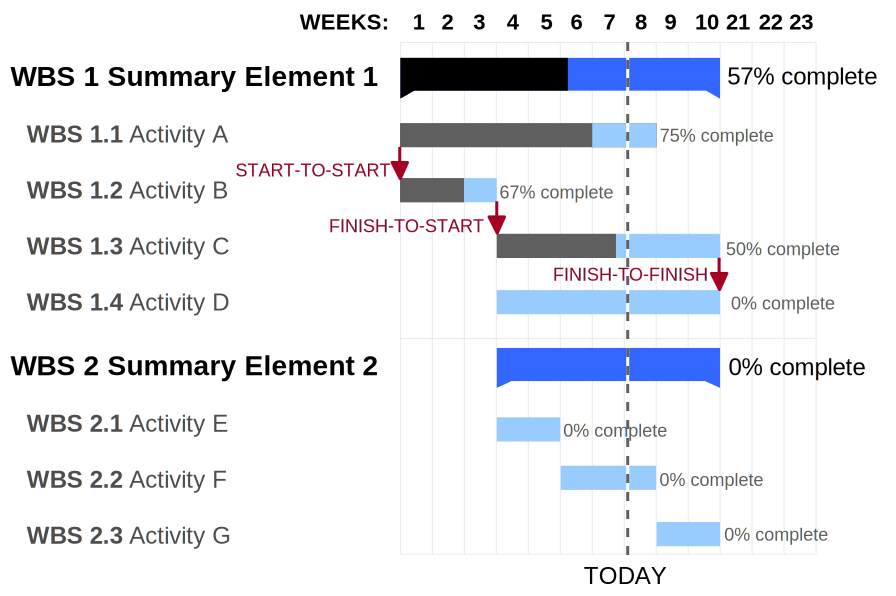
\includegraphics{Grafika/wykres-gantt.svg}

Do wyznaczenia optymalnej kolejności opracowano wiele algorytmów, zarówno dokładnych jak i przybliżonych, z których najważniejsze to:

* Johnsona
* Campbella-Dudka-Smitha
* Browna-Łomnickiego

Wspomniane algorytmy zostaną omówione na przykładzie obróbki m detali na n maszynach. Dodatkowo, poniżej zostały sprecyzowane założenia, które muszą być spełnione:

* każdy detal jest obrabiany dokładnie raz na każdej maszynie
* czasy obróbki każdego detalu na każdej maszynie są znane
* nie można rozpocząć procesu obróbki kolejnego detalu zanim nie zostanie zakończony poprzedni
* kolejność procesu obróbki jest identyczna dla wszystkich detali z danej partii oraz każdej maszyny
 
Algorytm Johnsona

Wspomniany algorytm możliwy jest do użycia tylko w wypadku kiedy mamy 2 lub 3 maszyny do obróbki detali oraz poniższą macierz z czasami obróbki 

\begin{pmatrix} t_{1,1} & t_{1,2} & \cdots & t_{1,j} \\ t_{2,1} & t_{2,2} & \cdots & t_{2,j} \end{pmatrix}

1) Znajdujemy min t_{i,j}
2) Jeżeli min t_{i,j} = t_{1,k} to optymalna kolejność musi się rozpocząć od obróbki detalu o indeksie k natomiast jeżeli min t_{i,j} = t_{2,s} to musi zakończyć się detalem o indeksie s
3) Wykreślamy z powyższej macierzy czasów, kolumnę i ze znalezionym w drugim kroku minimum oraz wracamy do pierwszego kroku zakładając że znaleziony min t_{i,j} ustawia się w pierwszym wolnym miejscu, odpowiednio od końca lub początku.

Algorytm Campbella-Dudka-Smitha

Bazujący na algorytmie Johnsona, pozwala na znalezienie przybliżonej, optymalnej kolejności dla więcej niż 3 maszyn. W tym celu konstruuje się n-1 zadań pomocniczych zgodnie z poniższymi wzorami.

M_{1j}^r = \sum_{\small{i=1}}^{\small{r}} t_{ij}
M_{2j}^r = \sum_{\small{i=n+1-r}}^{\small{n}} t_{ij}

Wielkość M_{1j}^r odpowiada t_{1,j}, natomiast M_{2j}^r odpowiada t_{2,j} w algorytmie Johnsona. Po wykonaniu wszystkich kroków, wśród przybliżonych rozwiązań szukamy najlepszego metodą przeglądu zupełnego.

Algorytm Browna-Łomnickiego

Jest to algorytm dokładny, oparty o metodę podziału i ograniczeń. Do rozwiązania problemu przydatny jest graf, którego węzłami są indeksy kolejnych wariantów, a krawędzie mają przypisaną wartość max(g^1,g^2,...,g^n), gdzie g^1,g^2,...,g^n są wyliczone zgodnie z poniższym wzorem dla każdego z wariantów w każdym rzędzie

g^1 = T(i,w) + \sum_{\small{j \not\in w}} t_{ij} + \min_{\small{j \not\in w}} \sum_{\small{l=i+1}}^{\small n} t_{lj}
g^n = T(n,w) + \sum_{\small{j \not\in w}} t_{nj}

I = zbiór numerów wyrobów = {1,2,3,…, m}
W = dowolny podzbiór I
T(i,w) = czas wykonania zbioru w na i-tym stanowisku

Analizując przygotowany graf znajdujemy optymalne rozwiązanie problemu harmonogramowania.
